\section{Data Acquisition and Trigger}
The LHC provides pp collisions with a bunch spacing of 25\ns, which corresponds to a rate of 40 MHz. With multiple collisions occurring per bunch crossing, the event rate incident upon CMS is much higher than 40 MHz. The maximum final event rate needs to average on the order of 1 kHz, limited by the storage and data acquisition. In order to reduce the event rate while maintaining a high efficiency of selecting interesting physics processes, CMS uses a trigger system to make quick calculations and decisions about which events to keep or discard. 

\subsection{Trigger}
The trigger systems are a two-stage decision-making tool, which reduce the event rate based on trigger primitives at varying levels of complexity. The stages of the trigger system are the Level One (L1) trigger and the and the High-Level Trigger (HLT)\cite{Khachatryan:2016bia}. 

The L1 trigger resides on custom boards with field-programmable gate arrays (FPGAs). These contain pattern recognition algorithms that are able perform rough calculations to create candidate tracks and calorimeter clusters used for classification. The L1 operates with a latency of 3.8 $\mathrm{\mu s}$ per event, and full detector readout is held in a buffer while the L1 decision is made. L1 objects are energy clusters from ECAL and HCAL and muon track segments. Decisions are based on rough reconstrution of objects such as electrons, photons, muons, jets, and \met.  Information flow in the L1 trigger is shown in Figure~\ref{fig:l1_trigger}. The output rate of the L1 is limited to 100 kHz. Events which pass the L1 trigger are used to seed the more robust HLT analysis\cite{Khachatryan:2016bia}. 

\begin{figure}[htb]
\centering
  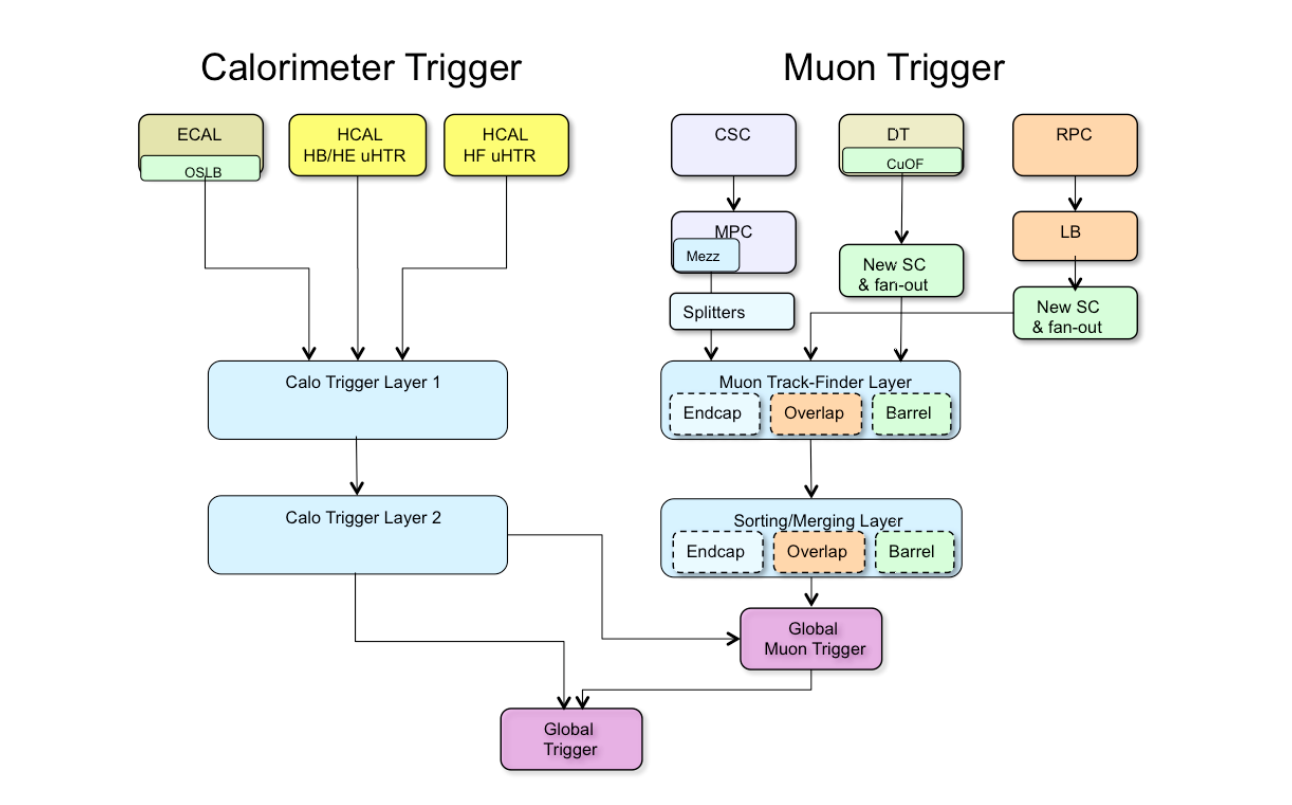
\includegraphics[width=0.75\linewidth]{plots/CMS/l1.PNG} 
  %https://cds.cern.ch/record/40524
  \caption{Schematic workflow of the L1 trigger. Information is first processed by the calorimeter and muon triggers, then combined at a global trigger \protect\cite{Cadamuro:2017slr}.}
  \label{fig:l1_trigger}
\end{figure}

The HLT system is a processor farm containing $O(10,000)$ CPU cores \cite{Adam:2005zf}. Here, fragments of events are combined to form complete events. The algorithms used to perform event reconstruction at the HLT level produce a similar quality as those used in the offline reconstruction, and the HLT has access to the full event readout. HLT reconstruction is seeded by the L1 trigger decision. HLT paths allow for quick reconstruction by selectively filtering events as the reconstruction steps proceed---decisions are based on easily reconstructable calorimeter clusters or muon tracks, while computationally expensive track finding is only performed on events which pass the other criteria. Events passing selection by the HLT are saved to be fully reconstructed and stored for analysis use. The average event selection rate by the HLT is 1000 Hz \cite{Khachatryan:2016bia}. 

\subsection{Data Storage and Processing}
Those events which pass the HLT filtering are stored on disk and eventually transferred to a Tier-0 computing center for full offline reconstruction and permanent storage. Data is stored and processed in part of a global computing grid, with multiple copies of datasets stored at computing centers around the world. 
%%%%%%%%%%%%%%%%%%%%%%%%%%%%%%%%%%%%%%%%%%%%%%%%%%%%%
%%%%%%%%%%%%%%%%%%%%%%%%%%%%%%%%%%%%%%%%%%%%%%%%%%%%%
\section{Detector Simulation}
Physical processes originating at the pp collision point are simulated by a series of event generators, which are described in a later chapter. In addition to generating the pp collision products, the simulated event sets must also incorporate effects due to the full chain of particle interactions and detector readout in CMS.

Particle propagation through the detector volume is modeled by GEANT4\cite{AGOSTINELLI2003250}. This toolkit allows a full geometric reconstruction of the detector, and handles the particle transport through the materials. Particle decays, bremsstrahlung, electromagnetic interactions, and hadronic interactions with the materials are modeled, as well as the effect of the magnetic field \cite{ALLISON2016186}. GEANT4 also handles detector response simulation, i.e. the simulation of optical photon production in a scintillator. Readout electronics, including associated noise, are also simulated.

Following the simulation of detector readout electrons, the simulated information is in the same format as data collected by the detector. At this stage, the full CMS reconstruction is applied to the simulation in the same way it is applied to data. 
%%%%%%%%%%%%%%%%%%%%%%%%%%%%%%%%%%%%%%%%%%%%%%%%%%%%%
%%%%%%%%%%%%%%%%%%%%%%%%%%%%%%%%%%%%%%%%%%%%%%%%%%%%%

\section{Luminosity Calibration}\label{ch:cms:lumi}
An accurate luminosity measurement is necessary to provide an estimate of the correct production yield for the W and Z bosons. Luminosity calibration at CMS is calculated by readout from dedicated luminosity monitors, rates of reconstructed objects in CMS, and dedicated LHC configurations to perform Van der Meer scans.

During LHC operation, measurement of \phil{the} instantaneous luminosity is based on the event rate recorded by several detectors. Online luminosity information is provided by dedicated luminometers---the Pixel Luminosity Telescope (PLT), Fast Beam Conditions Monitor, and the HCAL Forward calorimeter (HF)---which are operated on a separate readout from CMS physics data. Offline luminosity monitoring is based on data collected by CMS: rates of reconstructed pixel cluster counts and rates of tracks in the muon drift tubes\cite{Lujan:2647819}.

Absolute calibration is determined by a Van der Meer (VdM) scan \cite{vanderMeer:1968zz}\cite{Balagura:2011yw}, which utilizes a dedicated LHC configuration to scan the opposing proton beams transversely across each other. Data collected by CMS during these scans is used to reconstruct a beam profile and to determine the relationship of the instantaneous luminosity to the rates measured by the various luminosity monitoring systems.

Uncertainties in the luminosity measurement come from two primary categories. Normalization uncertainties, treated as uncorrelated, come from uncertainties of length scales and correlations when performing VdM scans. Integration uncertainties are related to detector operation and nonlinear detector response corrections\cite{CMS:2018elu}.